\documentclass[11pt, tikz, border=10pt]{standalone}
\usepackage{pgfplots}
\pgfplotsset{compat=1.18}
\usetikzlibrary{calc, arrows.meta, positioning, shapes.geometric, fit}

\definecolor{bglight}{HTML}{F8FAFC}
\definecolor{borderc}{HTML}{E2E8F0}
\definecolor{textmain}{HTML}{0F172A}
\definecolor{textsub}{HTML}{475569}
\definecolor{chartblue}{HTML}{0284C7}
\definecolor{queryred}{HTML}{EF4444}
\definecolor{valleygreen}{RGB}{35,95,25}
\definecolor{midgreen}{RGB}{95,155,100}
\definecolor{dirtbrown}{RGB}{185,150,110}
\definecolor{rockbrown}{RGB}{215,200,185}
\definecolor{snowwhite}{RGB}{250,250,250}

\begin{document}

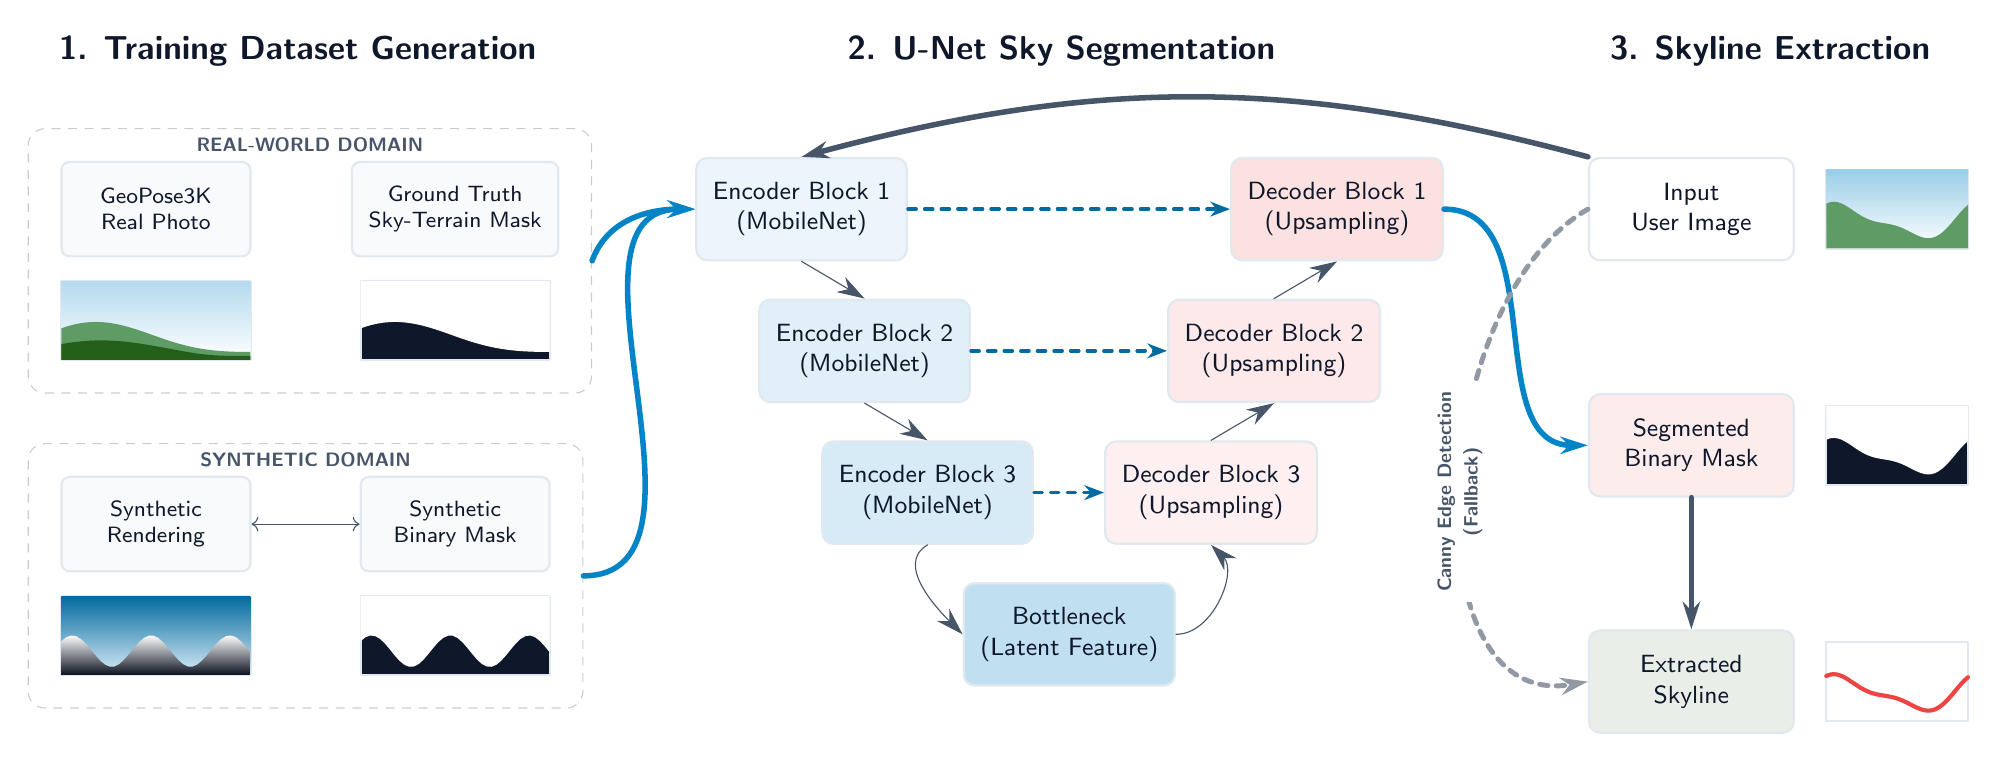
\begin{tikzpicture}[
    line join=round, 
    line cap=round,
    % Node styles
    boxstyle/.style={
        draw=borderc, thick, fill=white, rounded corners=4pt, 
        align=center, text=textmain, font=\sffamily\small,
        minimum width=2.6cm, minimum height=1.3cm,
        inner sep=6pt
    },
    datastyle/.style={
        draw=borderc, thick, fill=bglight, rounded corners=3pt,
        align=center, text=textmain, font=\sffamily\footnotesize,
        minimum width=2.4cm, minimum height=1.2cm,
        inner sep=6pt
    },
    arrowstyle/.style={
        -{Stealth[length=3.5mm, width=2.2mm]},
        line width=2pt,
        draw=textsub
    },
    skipstyle/.style={
        dashed,
        -{Stealth[length=2.5mm]},
        line width=1.2pt,
        draw=chartblue!80!black
    },
    fallbackstyle/.style={
        dashed,
        -{Stealth[length=3.5mm, width=2.2mm]},
        line width=1.8pt,
        draw=textsub!60
    },
    % Mathematical function representing the exact geographical skyline for the user image pipeline
    declare function={
        user_skyline(\x) = 0.35 + 0.20*sin(\x*200 + 45) + 0.08*cos(\x*380);
    }
]

    % ========================================================
    % SECTION A: TRAINING DATASET PIPELINE (Left Side)
    % ========================================================
    \node[font=\large\sffamily\bfseries, text=textmain] (title1) at (1.8, 9.5) {1. Training Dataset Generation};

    % Real Data Pipeline (Photo + Mask)
    \begin{scope}[local bounding box=realdata]
        % Real Photo
        \node[datastyle] (geophoto) at (0, 7.5) {GeoPose3K\\Real Photo};
        \begin{scope}[shift={($(geophoto.south) + (-1.2,-1.3)$)}]
            \draw[borderc, thick, fill=white] (0,0) rectangle (2.4, 1.0);
            \shade[top color=chartblue!30, bottom color=white] (0,0) rectangle (2.4, 1.0);
            \fill[midgreen] (0,0) -- (0, 0.4) to[out=20, in=160] (1.2, 0.3) to[out=-20, in=180] (2.4, 0.1) -- (2.4,0) -- cycle;
            \fill[valleygreen] (0,0) -- (0, 0.2) to[out=10, in=170] (1.6, 0.1) to[out=-10, in=180] (2.4, 0.05) -- (2.4,0) -- cycle;
        \end{scope}

        % Ground Truth Binary Mask
        \node[datastyle] (geomask) at (3.8, 7.5) {Ground Truth\\Sky-Terrain Mask};
        \begin{scope}[shift={($(geomask.south) + (-1.2,-1.3)$)}]
            \draw[borderc, thick, fill=textmain] (0,0) rectangle (2.4, 1.0);
            \fill[white] (0, 1.0) -- (0, 0.4) to[out=20, in=160] (1.2, 0.3) to[out=-20, in=180] (2.4, 0.1) -- (2.4,1.0) -- cycle;
        \end{scope}
    \end{scope}
    
    % Synthetic Data Pipeline (Horizon -> Rendering)
    \begin{scope}[local bounding box=synthdata]
        % Synthetic Renderings (Input to U-Net)
        \node[datastyle] (synthrender_img) at (0, 3.5) {Synthetic\\Rendering};
        \begin{scope}[shift={($(synthrender_img.south) + (-1.2,-1.3)$)}]
            \draw[borderc, thick, fill=white] (0,0) rectangle (2.4, 1.0);
            \shade[top color=chartblue!80!black, bottom color=chartblue!15!white] (0,0) rectangle (2.4, 1.0);
            \shade[top color=snowwhite, bottom color=textmain!80!black, draw=none] 
                (0,0) -- plot[domain=0:2.4, samples=40] (\x, {0.3 + 0.20*sin(\x*360 + 40)}) -- (2.4,0) -- cycle;
        \end{scope}

        % Synthetic Training Masks (Ground Truth for U-Net)
        \node[datastyle] (synthrender_mask) at (3.8, 3.5) {Synthetic\\Binary Mask};
        \begin{scope}[shift={($(synthrender_mask.south) + (-1.2,-1.3)$)}]
            \draw[borderc, thick, fill=textmain] (0,0) rectangle (2.4, 1.0);
            \fill[white] (0, 1.0) -- plot[domain=0:2.4, samples=40] (\x, {0.3 + 0.20*sin(\x*360 + 40)}) -- (2.4,1.0) -- cycle;
        \end{scope}

        \draw[arrowstyle, thin, <->] (synthrender_img) -- (synthrender_mask);
    \end{scope}

    % Group boxes
    \node[draw=textsub!30, dashed, inner sep=12pt, rounded corners=6pt, fit=(realdata)] (boxreal) {};
    \node[draw=textsub!30, dashed, inner sep=12pt, rounded corners=6pt, fit=(synthdata)] (boxsynth) {};
    \node[anchor=north, text=textsub, font=\sffamily\bfseries\scriptsize] at (boxreal.north) {REAL-WORLD DOMAIN};
    \node[anchor=north, text=textsub, font=\sffamily\bfseries\scriptsize] at (boxsynth.north) {SYNTHETIC DOMAIN};

    % ========================================================
    % SECTION B: STANDARD U-NET SCHEMATIC (Center)
    % ========================================================
    \node[font=\large\sffamily\bfseries, text=textmain] (title2) at (11.5, 9.5) {2. U-Net Sky Segmentation};

    \begin{scope}[shift={(8.2, 1.5)}]
        % Contracting Path (Encoder Blocks - kept at uniform 2.6cm)
        \node[boxstyle, fill=chartblue!8, minimum width=2.6cm] (enc1) at (0, 6.0) {Encoder Block 1\\(MobileNet)};
        \node[boxstyle, fill=chartblue!12, minimum width=2.6cm] (enc2) at (0.8, 4.2) {Encoder Block 2\\(MobileNet)};
        \node[boxstyle, fill=chartblue!16, minimum width=2.6cm] (enc3) at (1.6, 2.4) {Encoder Block 3\\(MobileNet)};
        
        % Bottleneck (Shifted horizontally to 3.4 for spacing)
        \node[boxstyle, fill=chartblue!25, minimum width=2.6cm] (bottleneck) at (3.4, 0.6) {Bottleneck\\(Latent Feature)};

        % Expanding Path (Decoder Blocks - shifted horizontally to start at 5.2 for a 1.0cm gap)
        \node[boxstyle, fill=queryred!8, minimum width=2.6cm] (dec3) at (5.2, 2.4) {Decoder Block 3\\(Upsampling)};
        \node[boxstyle, fill=queryred!12, minimum width=2.6cm] (dec2) at (6.0, 4.2) {Decoder Block 2\\(Upsampling)};
        \node[boxstyle, fill=queryred!16, minimum width=2.6cm] (dec1) at (6.8, 6.0) {Decoder Block 1\\(Upsampling)};

        % Encoder Downsampling Arrows (Clean, separated diagonal lines connecting blocks)
        \draw[arrowstyle, thin] (enc1.south) -- (enc2.north);
        \draw[arrowstyle, thin] (enc2.south) -- (enc3.north);
        \draw[arrowstyle, thin] (enc3.south) to[out=210, in=135] (bottleneck.west);

        % Decoder Upsampling Arrows (Clean, separated diagonal lines connecting blocks)
        \draw[arrowstyle, thin] (bottleneck.east) to[out=0, in=-45] (dec3.south);
        \draw[arrowstyle, thin] (dec3.north) -- (dec2.south);
        \draw[arrowstyle, thin] (dec2.north) -- (dec1.south);

        % Skip Connections (All lines, especially enc3 to dec3, are now clearly visible)
        \draw[skipstyle] (enc1.east) -- (dec1.west);
        \draw[skipstyle] (enc2.east) -- (dec2.west);
        \draw[skipstyle] (enc3.east) -- (dec3.west);
    \end{scope}

    % Dataset connection arrows to U-Net training phase (Kept unchanged)
    \draw[arrowstyle, chartblue] (boxreal.east) to[out=70, in=180] (enc1.west);
    \draw[arrowstyle, chartblue] (boxsynth.east) to[out=0, in=180] (enc1.west);

    % ========================================================
    % SECTION C: PIPELINE INFERENCE & EXTRACTION (Right Side)
    % ========================================================
    \node[font=\large\sffamily\bfseries, text=textmain] (title3) at (20.5, 9.5) {3. Skyline Extraction};

    % Inference Nodes - Primary Pipeline
    \node[boxstyle] (userimg) at (19.5, 7.5) {Input\\User Image};
    \node[boxstyle, fill=queryred!10] (segmask) at (19.5, 4.5) {Segmented\\Binary Mask};
    \node[boxstyle, fill=valleygreen!10] (extraction) at (19.5, 1.5) {Extracted\\Skyline};

    % Illustrative Thumbnail Assets (Now sharing a unified mathematical skyline function)
    % User Image Thumbnail
    \begin{scope}[shift={($(userimg.east) + (0.4,-0.5)$)}]
        \draw[borderc, thick, fill=white] (0,0) rectangle (1.8, 1.0);
        \shade[top color=chartblue!40, bottom color=white] (0,0) rectangle (1.8, 1.0);
        \fill[midgreen] (0,0) -- plot[domain=0:1.8, samples=40] (\x, {user_skyline(\x)}) -- (1.8,0) -- cycle;
    \end{scope}

    % Binary Mask Thumbnail
    \begin{scope}[shift={($(segmask.east) + (0.4,-0.5)$)}]
        \draw[borderc, thick, fill=textmain] (0,0) rectangle (1.8, 1.0);
        \fill[white] (0, 1.0) -- plot[domain=0:1.8, samples=40] (\x, {user_skyline(\x)}) -- (1.8,1.0) -- cycle;
    \end{scope}

    % Extracted Skyline Plot Thumbnail
    \begin{scope}[shift={($(extraction.east) + (0.4,-0.5)$)}]
        \draw[borderc, thick, fill=white] (0,0) rectangle (1.8, 1.0);
        \draw[queryred, line width=1.5pt] plot[domain=0:1.8, samples=40] (\x, {user_skyline(\x)});
    \end{scope}

    % Tightened U-Net input arrow (significantly reduced radius to prevent towering over titles)
    \draw[arrowstyle] (userimg.north west) to[out=165, in=15] (enc1.north);
    
    % U-Net Decoder -> Segmented Mask
    \draw[arrowstyle, chartblue] (dec1.east) to[out=0, in=180] (segmask.west);
    
    % Mask -> Extracted Skyline
    \draw[arrowstyle] (segmask) -- (extraction);

    % Direct Canny Edge Detection Fallback Bypass (Rerouted completely to the left of the inference stack)
    \draw[fallbackstyle] (userimg.west) to[out=210, in=190] 
        node[
            font=\sffamily\bfseries\scriptsize,
            text=textsub,
            fill=white,
            inner sep=3.5pt,
            rotate=90,
            anchor=center
        ] {\shortstack{Canny Edge Detection\\(Fallback)}}
    (extraction.west);

\end{tikzpicture}
\end{document}
